\documentclass[fullpage]{extarticle}
\usepackage[utf8]{inputenc}
\usepackage{cite}
\usepackage{fancyhdr}
\usepackage[margin=1in]{geometry}
\usepackage{setspace}
\usepackage{hyperref}
\usepackage{graphicx}
\usepackage{amsmath}
\usepackage{amsfonts}
\usepackage{textcomp}
\pagestyle{headings}

\doublespacing

\title{Modelling the Spread of SARS-CoV-2 using Small World Networks}
\author{
	Jordan R. Williams\\
	\texttt{jwilliams13@umassd.edu}
	\and
	Alana R. McGraw\\
	\texttt{amcgraw@umassd.edu}
}
\date{January 18, 2021}
\begin{document}

\maketitle
\begin{center}
MTH 465\\
\end{center}

\begin{large}
\begin{center}\bigbreak\bigbreak\bigbreak
ABSTRACT
\end{center}
\end{large}

\begin{large}
\begin{flushleft}
The COVID-19 pandemic has presented a major challenge for residential universities, as they try to balance the economic needs of the school and local community with the safety of faculty and staff. In this paper, we will be modeling the spread of SARS-CoV-2 on the University of Massachusetts Dartmouth campus in order to assess whether the safety protocols that are currently in place are viable for the future. We generated our model for the spread of SARS-CoV-2 using a Strogatz-Watts network ($n=1500$, $k=43$, $diameter=6$) in order to address the characteristics of the social network the disease would spread along, and using a complete graph ($n=1500$) to compare spread on a network that assumes homogenous mixing. We started a 100 day semester with 1500 uninfected and susceptible individuals, considering best (low rate of infection, 3 exogenous cases per week), base (mid-range rate of infection, 10 exogenous cases per week), and worst (high rate of infection, 15 exogenous cases per week) case models for how SARS-CoV-2 would spread in a homogenous population compared to our more realistic social network. Our base case, with screening every 1, 2, 3, 7 days, symptom-based, or not at all resulted in an average of 1500 cumulative cases per semester for all testing protocols with the complete graph and an average of 158.5, 169.7, 180.8, 280.4, 656.8, and 938.2 cumulative cases per semester for the Strogatz-Watts network, using the approximate sensitivity and specificity of the CRSP SARS-CoV-2 Real-time Reverse Transcriptase (RT)-PCR Diagnostic Assay. Our model demonstrated that testing every 3 days was the best option for preventing transmission of SARS-CoV-2 in a cost effective manner for each scenario, but testing every 1-7 days was generally adequate, and that assumptions of homogenous mixing dramatically increase expectations of disease spread. While this model was made with specific consideration of the protocols in place at the University of Massachusetts Dartmouth, it can be applied to other medium sized universities operating with similar no/low risk protocols.
\end{flushleft}
\end{large}

\begin{center}
\section{INTRODUCTION}
\label{sec:intro}
\end{center}

\begin{large}
\begin{flushleft}
In December of 2019, the first case of the COVID-19 illness was reported in China, and soon after the World Health Organization (WHO) characterized it as a Public Health Emergency of International Concern. As of November 23, 2020, there have been 14.7 million cases and over 281,878 deaths in the US; in Massachusetts alone there have been 252,017 cases [\hyperref[ref:1]{1}]. This global pandemic has presented a great challenge to colleges and universities around the world.  If schools are going to remain open, it is essential that they develop effective strategies in order to mitigate the spread of this disease. The severity of this public health threat, in conjunction with the threat of financial consequences if universities close, has made it imperative that schools develop effective plans for preventing the spread of SARS-CoV-2 on their campuses.\bigbreak
Universities around the country have developed testing strategies in order to balance the serious financial consequences of shutting their doors and public safety concerns. The University of Massachusetts Dartmouth has strict weekly testing protocols using the CRSP SARS-CoV-2 Real-Time Reverse Transcriptase (RT)-PCR Diagnostic Assay, which has been made available by the FDA with Emergency Use Authorization. Students, faculty, and staff that regularly visit campus are required to be tested once a week, wear face masks in all public spaces on campus, and buildings are operating at limited capacity with enhanced cleaning strategies.\bigbreak
Previous studies modelling the coronavirus spread on mid-sized university campuses have suggested that effective testing strategies include testing every 2 days with a low-sensitivity, high-specificity test. These models are limited because they assume that every individual will come into contact with one another on the campus [\hyperref[ref:10]{10}], but this does not consider the nature of human social interactions. Small world networks (SWN; e.g. Strogatz-Watts) are able to more accurately capture the high clustering and the relatively low diameter of real social networks. SWNs reflect that people are generally connected to groups of people that know one another, and that a few random connections make the path between two seemingly distant individuals relatively small. With an infectious virus like SARS-CoV-2, which spreads through contact, a SWN is a more realistic way to model disease spread.\bigbreak
In our model, we plan to consider a hypothetical cohort of 1500 students that are all susceptible to SARS-CoV-2. In this model, one node (or vertex) will represent one student on campus, and an edge between any two nodes in the network will signify that these students have some form of social interaction where the virus has the potential to spread. The vertex degree of each node is representative of the number of connections the student has with other people on campus. In our SWN, the average vertex degree $k$ is a weighted average calculated by assuming on third of the students are commuters who only come into contact with 30 people and that the remaining residential students interact with about 50 people. We will be simulating the spread of SARS-CoV-2 on a SWN and a complete graph with 1500 nodes in order to assess whether models that assume homogenous mixing, like the standard SEIR models, result in different testing recommentations. Considering that we will more accurately account for how SARS-CoV-2 spreads with the SWN and that we now have more information on the reproduction rates ($R_t$) and number of exogenous cases from the fall semester, this model will be a better indicator of the spread of the disease across campus compared to the standard SEIR-models that assume a homogenous mixing of individuals. This information will allow us to assess whether the UMass Dartmouth reopening strategy will continue to be an effective way to mitigate COVID-19 spread.\bigbreak\bigbreak
\end{flushleft}
\end{large}

\begin{center}
\section{METHODS}
\label{sec:2}
\end{center}

\begin{table}[p!]
\begin{Large}
\begin{center}
\begin{tabular}{|c||c|c|}\hline
Parameter 							& Value		& Reference			\\ \hline\hline
Compartments for the Initial Population	&			&					\\ \hline
Noninfected, susceptible 				& $1500$	& [\hyperref[ref:15]{15}]	\\ \hline
Infected, exposed, $I_{0}$			& $0$		& Assumption		\\ \hline
Time Horizon, $d$					& $100$		& Semester length	\\ \hline\hline
Disease Dynamics						&			&				\\ \hline
Mean incubation time, $i$				& $3$ days	& [\hyperref[ref:6]{6}] \\ \hline
Time to Recovery		& $14$ days	& [\hyperref[ref:9]{9}, \hyperref[ref:13]{13}]	\\ \hline
Probability of Symptoms given infection	& $0.85$	& [\hyperref[ref:4]{4}, \hyperref[ref:7]{7}, \hyperref[ref:15]{15}]	\\ \hline
Transmission Rate, $\beta$			& Dependent on $R_{t}$	& [\hyperref[ref:12]{12}]	\\ \hline\hline 
Scenarios							&			&\\ \hline
Effective $R_{t}$						&			&							\\ \hline
Best,	${R_{t}}_{0}$						& $1.05$	& [\hyperref[ref:12]{12}]		\\ \hline
Base, ${R_{t}}_{1}$					& $1.5$		& [\hyperref[ref:12]{12}]		\\ \hline
Worst, ${R_{t}}_{2}$					& $2.0$		& [\hyperref[ref:12]{12}]		\\ \hline
Exogenous infections per week,	$X$		&			&					\\ \hline
Best,	$X_{0}$						& $5$		& [\hyperref[ref:15]{15}], Assumption		\\ \hline
Base, $X_{1}$						& $10$		& Assumption		\\ \hline
Worst, $X_{2}$						& $15$		& [\hyperref[ref:15]{15}], Assumption\\ \hline\hline
Test Characteristics					&			&					\\ \hline
Test Sensitivity (true positive rate)	& $0.948$	& [\hyperref[ref:5]{5}] \\ \hline
Test Specificity (true negative rate)	& $0.956$	& [\hyperref[ref:5]{5}] \\ \hline
Cost per test							& $\$25$	& [\hyperref[ref:3]{3}]	\\ \hline
Time to test result			& $1$ day	& [\hyperref[ref:15]{15}]		\\ \hline

\end{tabular}
\caption{\label{table:parameters}Parameters.}
\end{center}
\end{Large}
\end{table}

\begin{large}
\begin{flushleft}
2.1. \textbf{Graph Generation.}

A small world network was generated using the Strogatz-Watts model for its simplicity in implementation and desirable SWN properties. These properties include a small graph diameter and high mean clustering coefficient [\hyperref[ref:14]{14}].
\bigbreak
The algorithm used to generate a Strogatz-Watts graph is as follows:
\begin{enumerate}
	\item Generate a regular lattice with $n$ vertices and $k$ nearest neighbors per vertex.\\
	\item Replace a random edge from the regular lattice with an edge between two randomly-chosen vertices.
	\item Repeat step 2 until a desired graph diameter is reached.
\end{enumerate}

Since this algorithm has extremely high runtimes ($O(n^2)$) for high $n$, the graph was generated once with our parameters $n = 1500, k = 43$ and saved to a file. It was then reused for further test and simulations instead of a new graph being generated each time.\bigbreak

2.2 \textbf{Simulation.}

Environment:
\begin{itemize}
	\item Each node has a state that represents one of the following statuses: Susceptible ($S_s$), Exposed ($S_e$), Infected asymptomatic ($S_{I_a}$), Infected symptomatic ($S_{I_s}$), and Recovered ($S_r$).\\
	\item Upon changing states, a node's internal day counter resets back to 0.\\
	\item Each node may be quarantined for a period $t_q$, during which they may not spread infection nor become exposed.
\end{itemize}
\bigbreak
At the start of each simulation, a list of nodes (i.e., the student population) is generated of size $n = 1500$. All nodes begin in state $S_s$. There are no initial infected students ($I_0 = 0$).\bigbreak

For $d = 100$ time steps representing 100 days, each node was then updated according to its state:
\begin{itemize}
	\item $S_e$: on day $3$ (mean incubation period $i$), move to state $S_{I_a}$.\\
	\item $S_{I_a}$: on day 10, move to state $S_r$ with probability $0.15$. Otherwise, move to state $S_{I_s}$ on day 12. For every day not in quarantine, spread infection.\\
	\item $S_{I_s}$: on day 5, move into quarantine for 5 days. On day 10, move into state $S_r$. If the testing method is symptom-based, take a virus test every day not in quarantine.
\end{itemize}

This model assumes that after $10$ days of infection, all individuals will either recover with probability $0.15$ or develop symptoms 2 days later (with probability $0.85$).\bigbreak

When an infected node spreads infection, it iterates through all its neighbors as defined by the Strogatz-Watts model. If neither node is quarantined and the neighbor is in status $S_s$, the neighbor will be successfully infected with probability $\beta$. These $\beta$ values were calculated through trial and error by matching the measured $R_t$ value with the desired $R_t$ value ($1.05$, $1.5$, or $2.0$) in a simulation without tests.\bigbreak

Six different testing protocols are used to compare total test costs and number of infected cases over the semester. Individuals are either tested daily, every 2 days, every 3 days, weekly, after showing symptoms, or not at all.\bigbreak

If the testing method is specified to be every $t$ days, then every $t$ time steps each node gets tested for the virus. The test has a sensitivity of $0.948$ (true positive rate) and specificity of $0.956$ (true negative rate). Test results are delayed by $1$ day before individuals react to them (e.g., moving into quarantine). If a node tests positive, they move into quarantine for $14$ days.\bigbreak

Every 7 days, $X$ exogenous cases are added to the environment. This is simulated by $X$ randomly chosen susceptible nodes ($S_s$) being moved into state $S_e$.\bigbreak

This simulation ran every combination of best ($\beta = 0.18\%, X = 5$), base ($\beta = 0.26\%, X = 10$), and worst case ($\beta = 0.35\%, X = 35$) parameters and testing rates (no tests, symptom-based, 7 days, 3 days, 2 days, 1 day).\\
\end{flushleft}
\end{large}

\begin{figure}[b!]
\begin{center}
	\label{fig1}
	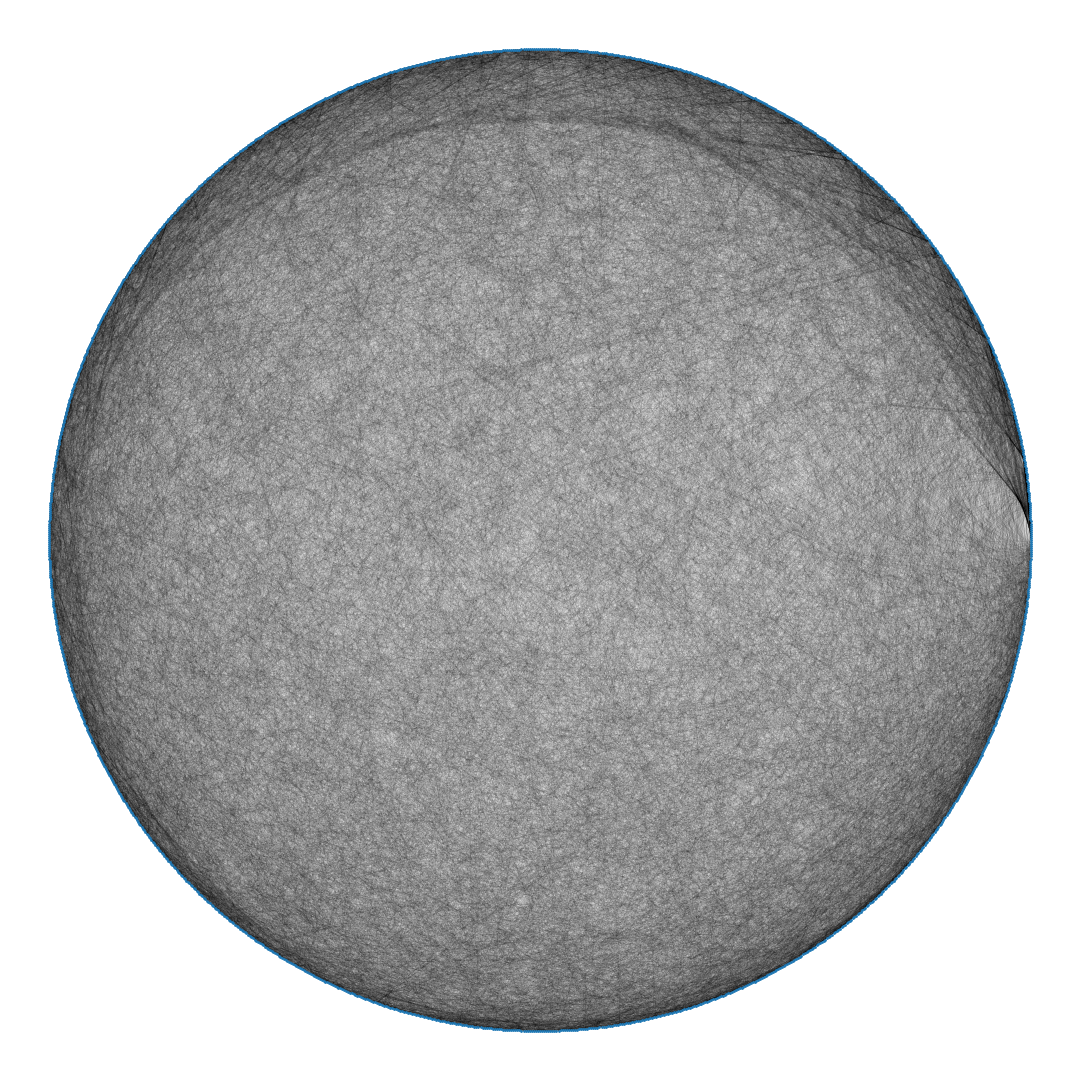
\includegraphics[width=\textwidth]{figures/ws/graph}
	\caption{The Strogatz-Watts graph ($n = 1500, k = 43, d = 6, CC = 0.72$) used in simulations.}
\end{center}
\end{figure}

\break

\begin{center}
\section{RESULTS}
\label{sec:3}
\end{center}


\begin{table}[b!]
\begin{Large}
\begin{center}
\begin{tabular}{|c||c|c||c|c|}\hline
Case 							&\multicolumn{2}{c||}{Complete Graph	}		&\multicolumn{2}{c|}{Small World Network}		\\  \cline{2-5}
 									&Cost (\$)			& Total Infected			&Cost (\$)			& Total Infected			\\ \hline\hline
Best Case 				&							&															&							&		\\ \hline
Daily 							& $2,378,948$					& $1387.6$ 				& $2,899,977$				&	$47.6$\\ \hline
Every 2 d					& $1,207,407$					& $1475.7$ 				& $1,419,079$				&	$50.6$\\ \hline
Every 3 d					& $884,311.50$				& $1499.8$ 				& $1,052,757$				&	$52.2$\\ \hline
Every 7 d					& $415,420$						& $1500$ 					& $480,279$					&	$68.9$\\ \hline
Symptom-based	& $318,440$						& $1500$ 					& $90,726.50$				&	$138.7$\\ \hline
None							& $0$									& $1500$ 					& $0$								&	$225.9$\\ \hline\hline
Base Case 				&							&															&							&		\\ \hline
Daily 							& $2,323,817$			& $1500$ 								& $2,181,257$			&	$158.5$\\ \hline
Every 2 d					& $1,214,665$			& $1500$ 								& $1,386,489$			&	$169.7$\\ \hline
Every 3 d					& $892,713$				& $1500$ 								& $1,024,919$			&	$180.8$\\ \hline
Every 7 d					& $410,278.50$		& $1500$ 								& $460,895$				&	$280.4$\\ \hline
Symptom-based	& $319,660$				& $1500$ 								& $444,075$				&	$656.8$\\ \hline
None							& $0$							& $1500$ 								& $0$							&	$938.2$\\ \hline\hline
Worst Case 			&							&															&							&		\\ \hline
Daily 							& $2,324,575$				& $1500$ 							& $2,753,794$				&	$238.5$\\ \hline
Every 2 d					& $1,221,617$				& $1500$ 							& $1,358,784$				&	$265.7$\\ \hline
Every 3 d					& $889,239$					& $1500$ 							& $999,731$					&	$286.3$\\ \hline
Every 7 d					& $415,847$					& $1500$ 							& $438,789.50$			&	$516.3$\\ \hline
Symptom-based	& $318,410$					& $1500$ 							& $914,204$					&	$111.2$\\ \hline
None							& $0$								& $1500$ 							& $0$								&	$1299.5$\\ \hline

\end{tabular}
\caption{\label{table:cases}Total cost and cases per semester for each scenario.}
\end{center}
\end{Large}
\end{table}

\begin{large}
\begin{flushleft}
We started the semester with a hypothetical cohort of 1500 students (approximately the number of students and faculty on the UMass Dartmouth Campus per week), all uninfected and susceptible to SARS-CoV-2. During a 100 day semester in the base case with 10 exogenous cases per week, screening every 1 to 7 days, symptom-based, or not at all on the SWN resulted in a range of 158.5 to 938.2 cumulative cases using the approximate sensitivity and specificity of the CRSP SARS-CoV-2 Real-time Reverse Transcriptase (RT)-PCR Diagnostic Assay. On the complete graph, all testing protocols lead to all 1500 students becoming infected in the base case. In the best case with 3 exogenous cases per week, the testing protocols used on the SWN resulted in 47.6 to 225.9 total cases per semester. On the complete graph, the total number of infected in the best case scenario ranged from 1387.6 to 1500 per sememester. In the worst case with 15 exogenous cases per week, the different testing strategies resulted in 238.5 to 1299.5 cumulative cases per semester on the SWN. On the complete graph, all testing protocols lead to 1500 total infected students for the worst case scenario. Table 2 and Figures 2, 3, and 4 illustrate the cumulative infections for each epidemic scenario, considering the frequency of testing and the graph type of the model.\bigbreak
 
With a price of \$25 per test, the overall cost of testing in each scenario was evaluated for the 6 different screening time protocols, for the complete graph and SWN models. The average cost of testing every day ranged from \$2,181,275 to \$2,899,977 in the best, base, and worst cases for the 100 day semester in the SWN; cost differences can be attributed to quarantined individuals not being tested. In the complete graph model, costs ranged from \$2,323,817 to \$2,378,948 for daily testing. The average cost of testing every 2 days was \$1,358,784 to \$1,419,079 for the SWN and \$1,207,407 to \$1,221,617 for the complete graph. The average cost of testing every 3 days was \$999,731 to \$1,052,757 for the SWN and \$884,311.50 to \$892,713 for the complete graph. The average cost of testing every 7 days was \$438,789.50 to \$480,279 for the SWN and \$410,278.50 to \$415,847 for the complete graph. The average cost of testing based on symptoms was \$90,726.50 to \$914,204 for the SWN and \$318,410 to \$319,660 for the complete graph. Finally, not testing at all had a trivial testing cost of \$0 for all 3 scenarios in both models.


\begin{figure}
\begin{center}
	\label{fig2}
	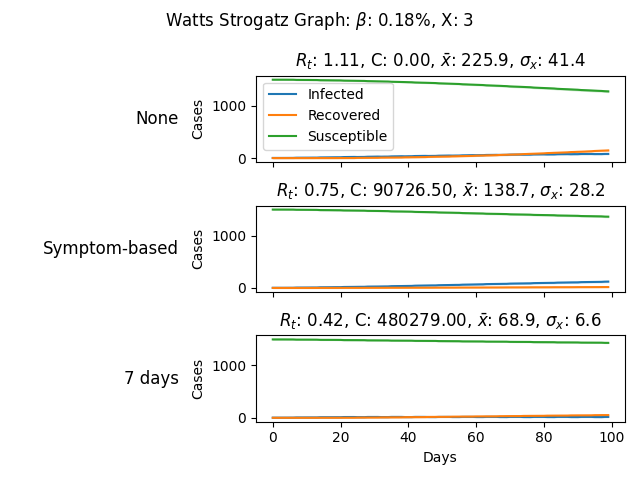
\includegraphics[width=0.85\textwidth]{figures/ws/results_best_none-symp-7}
	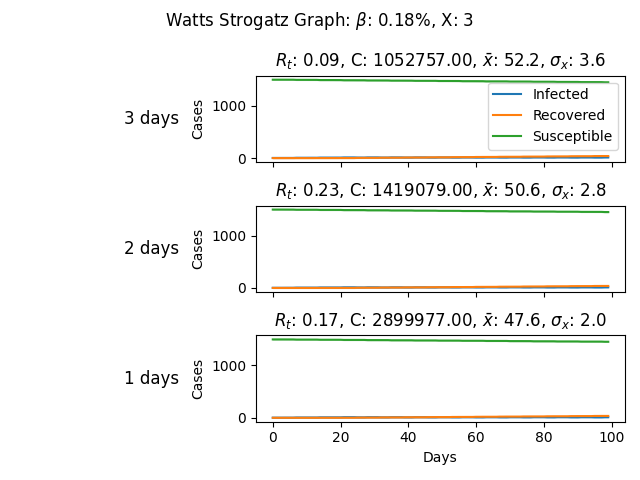
\includegraphics[width=0.85\textwidth]{figures/ws/results_best_3-2-1}
	\caption{Susceptible, infected, and recovered counts during best-case simulations with varying testing rates.}
\end{center}
\end{figure}

\begin{figure}
\begin{center}
	\label{fig3}
	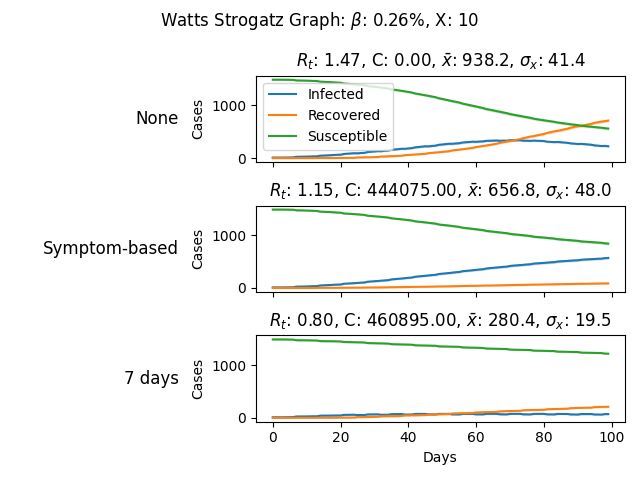
\includegraphics[width=0.85\textwidth]{figures/ws/results_base_none-symp-7}
	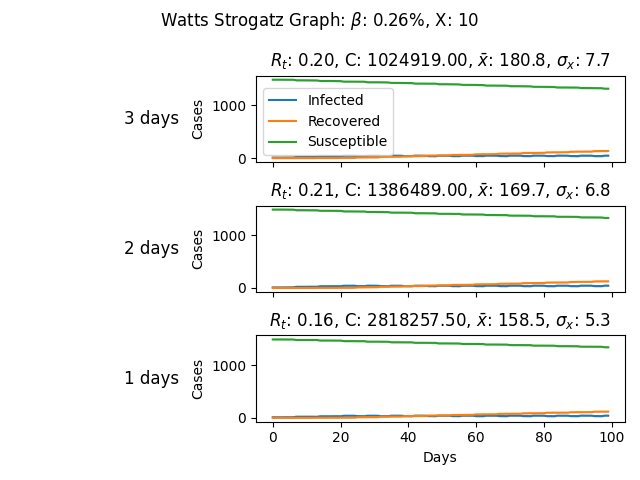
\includegraphics[width=0.85\textwidth]{figures/ws/results_base_3-2-1}
	\caption{Susceptible, infected, and recovered counts during base-case simulations with varying testing rates.}
\end{center}
\end{figure}


\begin{figure}
\begin{center}
	\label{fig4}
	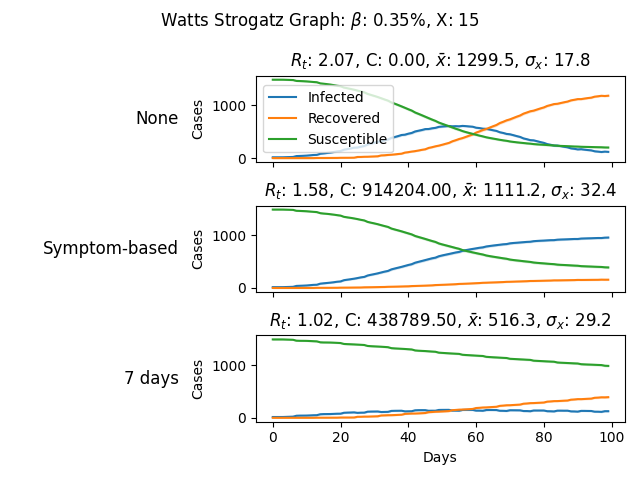
\includegraphics[width=0.85\textwidth]{figures/ws/results_worst_none-symp-7}
	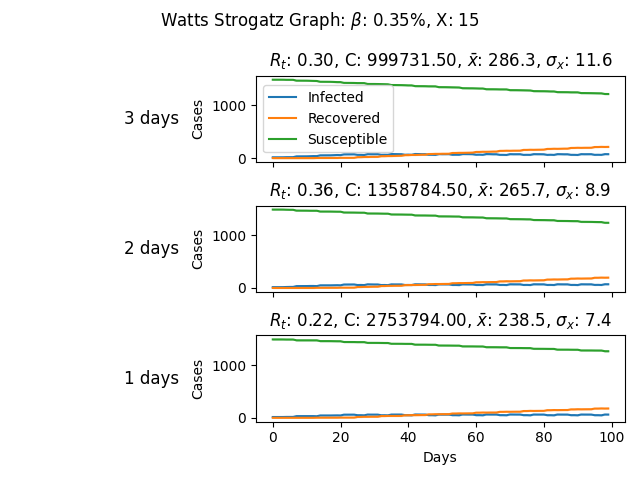
\includegraphics[width=0.85\textwidth]{figures/ws/results_worst_3-2-1}
	\caption{Susceptible, infected, and recovered counts during worst-case simulations with varying testing rates.}
\end{center}
\end{figure}

\end{flushleft}
\end{large}

\break

\begin{center}
\section{DISCUSSION}
\label{sec:4}
\end{center}

\begin{large}
\begin{flushleft}
Colleges and universities need effective testing strategies in order to operate safely, even if they are limiting the number of people coming onto campus. This model builds on previous studies by more accurately modelling how the virus would spread in a social network using a SWN (Strogatz-Watts) that captures the high clustering, and low diameter which is characteristic of real social networks, rather than assuming homogenous mixing [\hyperref[ref:10]{10}]. We found evidence that screening every 1-7 days would be adequate for buffering the transmission of SARS-CoV-2. Our model did not support symptom-based testing as a feasible or cost effective option for detecting and containing viral transmission. \bigbreak

As discussed earlier, testing every 2 days was identified as the best option for controlling the spread of SARS-CoV-2 on college campuses in a cost effective manner using the standard SEIR model [\hyperref[ref:10]{10}]. We found that testing every 3 days reduced total cost by about \$400,000 dollars compared to testing every 2 days with minimal increase in total cases. We also found that the protocol UMass Dartmouth uses, testing every 7 days, provided adequate protection for the best and base cases at a relatively low cost, but in the worst case led to over a third of the population on campus becoming infected. This information supports weekly testing, but we would suggest increasing the rate of testing if the circumstances defined in the worst case scenario come to pass. The worst case is based on the highest $R_t$ value (which translated into the highest infection rates, $\beta$) that was present in the state of Massachusetts, and the worst exogenous case number $X$ per week is based on the number of positive cases identified at UMass Dartmouth on the week of November 16, 2020 that did not result from internal spread; some assumptions were made to estimate which cases were truly exogenous [\hyperref[ref:12]{12}, \hyperref[ref:15]{15}].\bigbreak

Testing spread on the complete graph resulted in every student present on campus becoming infected in nearly every scenario. This is not what we expected, as we anticipated results closer to those found by Paltiel et al. This may indicate that our complete graph model does not properly incorporate the complexities of the SEIR model, but this issue can be addressed in future studies. Nevertheless, a comparison between the total number of cases in our SWN and complete graph model might suggest the overestimation of cases in models like SEIR that assume homogenous mixing of populations.\bigbreak

Our study was limited in assuming that the $R_t$ values for Massachusetts apply to the University of Massachusetts Dartmouth with all of the strict protocols in place, as protocols outside of campus grounds might be more lenient. These $R_t$ values were used to determine the infection rate ($\beta$) in each simulation. Most of the parameters that we are using, including $\beta$, the time it takes to get test results back, and the time of recovery are assumed to be static, but these parameters would change over time. We are also limited in our assumption that only 10 of the 35 cases identified at UMass Dartmouth on the week of 11/16/20 are exogenous and not from spread within the campus grounds. Our test specificity and sensitivity are also estimates from the 95\% confidence interval presented for the CRSP SARS-CoV-2 assay in the tests Emergency Use and Authorization summary [\hyperref[ref:5]{5}].\bigbreak

Reopening colleges and universities presents risk to not only the students but also the staff and faculty that come into close contact with each other, and the community as a whole if people leave campus infected and spread SARS-CoV-2 to their broader social network. Safety should be the biggest consideration decision makers on campus have, but we also recognize the financial balance that is required to keep schools operating into the future. Our model supports that there is a safe and cost effective way to keep universities open with proper safety and testing protocols.

\end{flushleft}
\end{large}
\pagebreak

\begin{center}
\section*{REFERENCES}
\label{sec:ref}
\end{center}

\begin{enumerate}
	\item \label{ref:1}Almukhatar, S., Sufrichtig, A., Barnard, A. Bloch, M., Calderone, J., et al. Covid in the US: 
Latest Map and Case Count. The New York Times. November 23, 2020.\hfill\break
	Accessed November 23, 2020.\hfill\break
	\url{https://www.nytimes.com/interactive/2020/us/coronavirus-us-cases.html#states}
	\item \label{ref:2}Bahl, R., Eikmeier, N., Fraser, A., Junge, M., Keesing, F., Nakahata, K., Wang, L.Z. Modeling 
covid-19 spread in small colleges. Cornell University. 2020.\hfill\break
	\url{https://arxiv.org/abs/2008.09597}
	\item \label{ref:3}Broad Communications. Broad Institute provides COVID-19 screening for students, faculty, and 
staff at more than 100 colleges and universities. Broad Institiute. 2020.\hfill\break
	\url{https://www.broadinstitute.org/news/broad-institute-provides-covid-19-screening-students-faculty-and-staff-more-100-colleges-and}
	\item \label{ref:4}Day M. COVID-19: four-fifths of cases are asymptomatic, China figures indicate. BMJ. 
2020;369:m1375. Doi:10.1136/bmj.m1375
	\item \label{ref:5}FDA. Emergency Use and Authorization (EUA) Summary CRSP SARS-CoV-2 Real-time 
Reverse Transcriptase (RT)-PCR Diagnostic Assay Clinical Research Sequencing Platform (CRSP), LLC at the Broad Institute of MIT and Harvard. 2020. U.S. Food and Drug Administration.\hfill\break
	\url{https://www.fda.gov/media/139858/download}
	\item \label{ref:6}He X, Lau EHY, Wu P, et al. Temporal dynamics in viral shedding and transmissibility of 
COVID-19. Nat Med. 2020;26(5):672-675. doi:10.1038/s41591-020-0869-5
	\item \label{ref:7}Ing AJ, Cocks C, Green JP. COVID-19: in the footsteps of Ernest Shackleton. Thorax. Published 
online May 27, 2020; thoraxjnl-2020-215091. doi:10.1136/thoraxjnl-2020-215091
	\item \label{ref:8}Ivorra, B., Ferrandez, M.R., Vela-Perez, M., and Ramos, A.M. Mathematical modeling of the 
spread of the coronavirus disease (COVID-19) taking into account the undetected infections. The case of China. Commun Nonlinear Sci Numer Simul. 2020.\hfill\break
	Doi: \url{https://dx.doi.org/10.1016\%2Fj.cnsns.2020.105303}
	\item \label{ref:9}Lauer SA, Grantz KH, Bi Q, et al. The incubation period of coronavirus disease 2019 
(COVID-19) from publicly reported confirmed cases: estimation and application. Ann Intern Med. 2020;172(9):577-582. doi:10.7326/ M20-0504
	\item \label{ref:10}Paltiel, D.A., Zheng, A., Walensky, R.P. Assessment of SARS-CoV-2 Screening Strategies to 
Permit the Safe Reopening of College Campuses in the United States. JAMA Network Open. 2020;3(7):e2016818. doi:10.1001/jamanetworkopen.2020.16818
	\item \label{ref:11}Preble, M. Returning to UMassD: Fall 2020 Reopening Plan. UMass Dartmouth. 2020.\hfill\break
	\url{https://www.umassd.edu/media/umassdartmouth/news/2020/UMassD-Fall-2020-Re-Opening-Plan.pdf}
	\item \label{ref:12}Shi, A., Ganyor, S., Li, X., Li, H., Li, Z., Shyr, D., Lin, X. Visualizing COVID-19’s Effective 
Reproduction Number (Rt). GitHub. 2020.\hfill\break
	\url{http://metrics.covid19-analysis.org/}
	\item \label{ref:13}US Centers for Disease Control and Prevention. COVID-19 pandemic planning scenarios. 
Updated May 20, 2020. Accessed July 7, 2020.\hfill\break
	\url{https://www.cdc.gov/coronavirus/2019-ncov/hcp/planning-scenarios.html}
	\item \label{ref:14}Watts DJ, Strogatz SH (1998) Collective dynamics of ‘small-world’ networks. Nature 393:4\hfill\break
	\url{https://www.nature.com/articles/30918.}
	\item \label{ref:15}Yan, D. COVID-19 Dashboard. UMass Dartmouth. November 19, 2020.\hfill\break
	\url{http://www.math.umassd.edu/~dyan/dashboard.html}
	\item \label{ref:16}Yang R, Gui X, Xiong Y. Comparison of clinical characteristics of patients with asymptomatic vs 
symptomatic coronavirus disease 2019 in Wuhan, China. JAMA Netw Open. 2020;3(5):e2010182. doi:10.1001/ jamanetworkopen.2020.10182

\end{enumerate}

\end{document}
